\chapter{Quantum error correction codes}
\section{Condition for quantum error correction}
In the previous sections we saw how the noise impact on the system, and how we can find a recovery procedure to correct an eventual error. However, there are some conditions to be able to recover a state affected by errors. These conditions are called Knill-Lafflame conditions and tell us when we can create a quantum error correcting code that is able to detect and correct the error.



In any code, we must never confuse the logical encoded qubits $|\overline{0}\rangle_L$ with $|\overline{1}\rangle_L$, even in the presence of errors.
Suppose, in fact, that two errors $E_a$ and $E_b$ map the initially orthogonal codewords $\ket{\overline{0}} \to E_a\ket{\overline{0}}$ and $\ket{\overline{1}} \to E_b \ket{\overline{1}}$ such that the faulty states have non-zero overlap : $\bra{\overline{1}}E_b^{\dagger}E_a\ket{\overline{0}} \neq 0$. 
When trying to detect the error that happened it is possible (non-zero probability) that we can not distinguish between the events where the system started. In other words, no measurement can decide with certainty whether the initial state was $\ket{0}_L$ or $\ket{1}_L$
If two codewords are orthogonal, and they are acted upon by correctable errors, the result will remain orthogonal. This is a necessary condition given a set $\mathcal{E}$ of correctable errors \footnote{Recall: a set $\mathcal{E}$ of correctable errors exist an operator $\mathcal{R}$ such that $\ket{\psi} = \mathcal{R}E\ket{\psi} \quad \forall E \in \mathcal{E}$}:
\begin{equation*}
    \bra{\overline{\psi_i}}E_b^{\dagger}E_a\ket{\overline{\psi_j}} = 0 \quad \forall E \in \mathcal{E} \text{   and   } \forall \ket{\psi_i} \neq \ket{\psi_j} \in \mathcal{C}
\end{equation*}
where $\mathcal{C}$ indicate the codespace.

This is not enough, another condition is required:
\begin{equation*}
    \bra{\overline{\psi_i}}E_b^{\dagger}E_a\ket{\overline{\psi_i}} = \bra{\overline{\psi_j}}E_b^{\dagger}E_a\ket{\overline{\psi_j}} \quad \forall E \in \mathcal{E} \text{   and   } \forall \ket{\psi_i},\ket{\psi_j} \in \mathcal{C}
\end{equation*}
This second condition is that the outcome of the syndrome measurement must not give any information about the codewords, otherwise the superposition state will collapse. 
whatever the state encoded in the subspace is, errors occurring on this state must not reveal anything about the state (otherwise we could learn something about the state, thereby destroying quantum information). In other words, the 'symmetric' inner product cannot depend on what exactly the 'current' codeword.
This two conditions, called also Knill-Lafflame conditions, can be combined in one yielding to the following theorem: 
 \begin{theorem}
 Suppose $\mathcal{E}$ is a linear space of errors acting on the Hilbert space
$\mathcal{H}$. Then a subspace $C$ of $\mathcal{H}$ forms a quantum error-correcting code correcting the errors $\mathcal{E}$ iff:
\begin{equation}
\bra{\psi_i}E_b^{\dagger}E_a\ket{\psi_j} = C_{a b}\delta_{ij}
\end{equation}
for all $E \in \mathcal{E}$. The matrix's elements $C_{a b}$ do not depend on the codewords $|\psi\rangle$.
\end{theorem}

Here $C_{a b}$ elements are constants independent of the codewords. Since $\bra{\psi_i}E_b^{\dagger}E_a\ket{\psi_j}=\left(\bra{\psi_i}E_a^{\dagger}E_b\ket{\psi_j}\right)^{*}$ for all $i$, we may write $C_{a b}$ as a Hermitian matrix.
If $C_{a b}$ has maximal rank, we say that the code is non-degenerate. Otherwise, if $C_{a b}$ has non-maximal rank, we say that the code is degenerate. A non-degenerate code refers to the case that each error in the set $\mathcal{E}_{c}$ corresponds to a unique syndrome, while in the case of degenerate code, there exist two errors in $\mathcal{E}_{c}$ whose syndromes are the same. For example, in the 9-qubit code is a degenerate code since the errors $Z_{1}, Z_{2}$, and $Z_{3}$ all have the same syndromes. Anyhow, applying $Z$ operation on any qubit in the first block can correct these errors.

\section{No-Cloning theorem}
In classical comunication we can copy a bit without any problem. This is one of the basic strategies for the classical error correction code, we increase the reliability of the code and then if a bit has been flipped, through a majority vote we can restore the information.  

Unfortunately, in quantum mechanics we are not allow to copy an unknown quantum state. This is due to the No-Cloning theorem [12], which states that it is not possible to copy an arbitrary pure quantum state into another. Moreover, a generalisation of the No-cloning theorem is the No-Brodcasting theorem which start from mixed states.
The impossibility to copy an arbitrary quantum state means that there is no unitary transformation that can copy an arbitrary state from the system A to the system B:
\begin{theorem}
There is no unitary operator $U$ on $\mathcal{H} \otimes H$ such that for all normalised states $|\psi\rangle_{A}$ and $|s\rangle_{B}$ in $H$
$$
U\left(|\psi\rangle_{A}|s\rangle_{B}\right)=e^{i \alpha(\psi, c)}|\psi\rangle_{A}|\psi\rangle_{B}
$$
for some real number $\alpha$ depending on $\psi$ and $s$.
\end{theorem}

\begin{proof}
Suppose we have two quantum systems $A$ and $B$.
We start from an unknown but pure quantum state in 
A, $|\psi\rangle_A$. This is the state which is to be copied in $B$. We assume that the target slot starts out in some standard pure state, $|s\rangle$. Thus the initial state is:
$$
|\psi\rangle \otimes|s\rangle .
$$
Then we would an unitary time-evolution operator $U$ that effects the copying procedure, ideally,
$$
\ket{\psi}\otimes|s\rangle \stackrel{U}{\longrightarrow} U(|\psi\rangle \otimes|s\rangle)=e^{i\alpha_{\psi}}|\psi\rangle \otimes|\psi\rangle
$$
It looks like that we actually performed the copying procedure for the state $\ket{\psi}$, however this procedure has to work for any state and not only for a specific state. 
Suppose then, this copying procedure works for two particular pure states, $|\psi\rangle_A$ and $|\varphi\rangle_A$. Then we have
$$
\begin{array}{c}
U(|\psi\rangle \otimes|s\rangle)=e^{i\alpha_{\psi}}|\psi\rangle \otimes|\psi\rangle \\
U(|\varphi\rangle \otimes|s\rangle)=e^{i\alpha_{\varphi}}|\varphi\rangle \otimes|\varphi\rangle
\end{array}
$$
The inner product of these two equations gives
\begin{align*}
    \bra{s}\bra{\varphi}U^{\dagger}U|\psi\rangle|s\rangle &= e^{i(\alpha_{\psi} -\alpha_{\varphi})}(\bra{\varphi}\bra{\varphi})(\ket{\psi}\ket{\psi})
    \\
    \langle\psi \mid \varphi\rangle&= e^{i(\alpha_{\psi} -\alpha_{\varphi})}(\langle\psi \mid \varphi\rangle)^{2}
\end{align*}
We can then take the absolute value of the last expression, and the phase factor vanish: 
\begin{equation*}
     |\langle \psi \mid \varphi\rangle|=|\langle\psi \mid \varphi\rangle|^{2}
\end{equation*}
But $x=x^{2}$ has only two solutions, $x=0$ and $x=1$, so either $|\psi\rangle=e^{i\gamma}|\varphi\rangle$ or $|\psi\rangle \perp |\varphi\rangle$. This means that we can theoretically clone only a precise state and its orthogonal states. However, this cannot be the case for two arbitrary states. Therefore, a single universal $U$ cannot clone a general quantum state. This proves the no-cloning theorem. 
\end{proof}


Further consideration can be done. The no cloning theorem states that it is not possible to perfectly cone the state but as shown in [13] it is possible to get an optimal copy of a state with certain fidelity. In addition, a different proof can be given showing that the No-cloning theorem works with mixed states as well; in this case, the theorem is often known as the No-broadcasting theorem
The no-cloning theorem prevents the use of certain classical error correction techniques on quantum states. For example, backup copies of a state in the middle of a quantum computation cannot be created and used for correcting subsequent errors.
Hence, we cannot use the classical "copy and paste" tactic in quantum error correction codes to protect our information, but this does not mean that we have to get rid of the classical error correction theory; indeed it is very helpful to build reliable code with minimum effort, for instance the CSS codes.
In quantum error correction another strategy is adopted: the information is not copied but it is spread out on multiple qubit. 


One of the simplest and emblematic quantum error correcting code that show this property is the 3-qubit code, although it can correct only a bit flip ($\sigma_X$) error, it is still a good starter point for more complicated algorithms.

\section{3-qubit error correction code}
% Unfortunately with quantum systems we cannot copy an unknow state, like the non-cloning theorem states. In other words, we cannot copy the same information about the system like in the classical case, where if we wanted to send a bit, we could have copied. 
% Instead, if we deal with quantum systems, we have to spread the information about the system among some qubits.
% Hence, in order to protect the original information we need to entangled it with some qubit. 

% The most basic quantum error correction code is the 3-Qubit code. This algorithm protects the information along a noisy channel that can affect the qubits with bit-flip error. However, before starting we need to make some assumptions about the noise: 
% \begin{itemize}
%     \item The noise 
%     \item The probability that the noise might flip a qubit  is ($p<\frac{1}{2}$)\footnote{This assumption is important when a fidelity check}
% \end{itemize}
Suppose that Alice wishes to transmit a qubit through a noisy channel to Bob, which leaves the qubit untouched with probability $1-p$, and flips the qubits with probability $p$ introducing a bit-flip $X$ error.

Before analysing the algorithm we need to make some assumptions about the noise: it acts on each qubit independently, it is identically distributed on each qubit, the quantum gates in the encoding and the decoding procedure are not subjected to errors and the probability $p$ has to be less than $\frac{1}{2}$ to be able to correct the error.



The quantum error correction method is summarised in figure \ref{fig:3fq}.
\begin{figure}[h!]
    \centering
    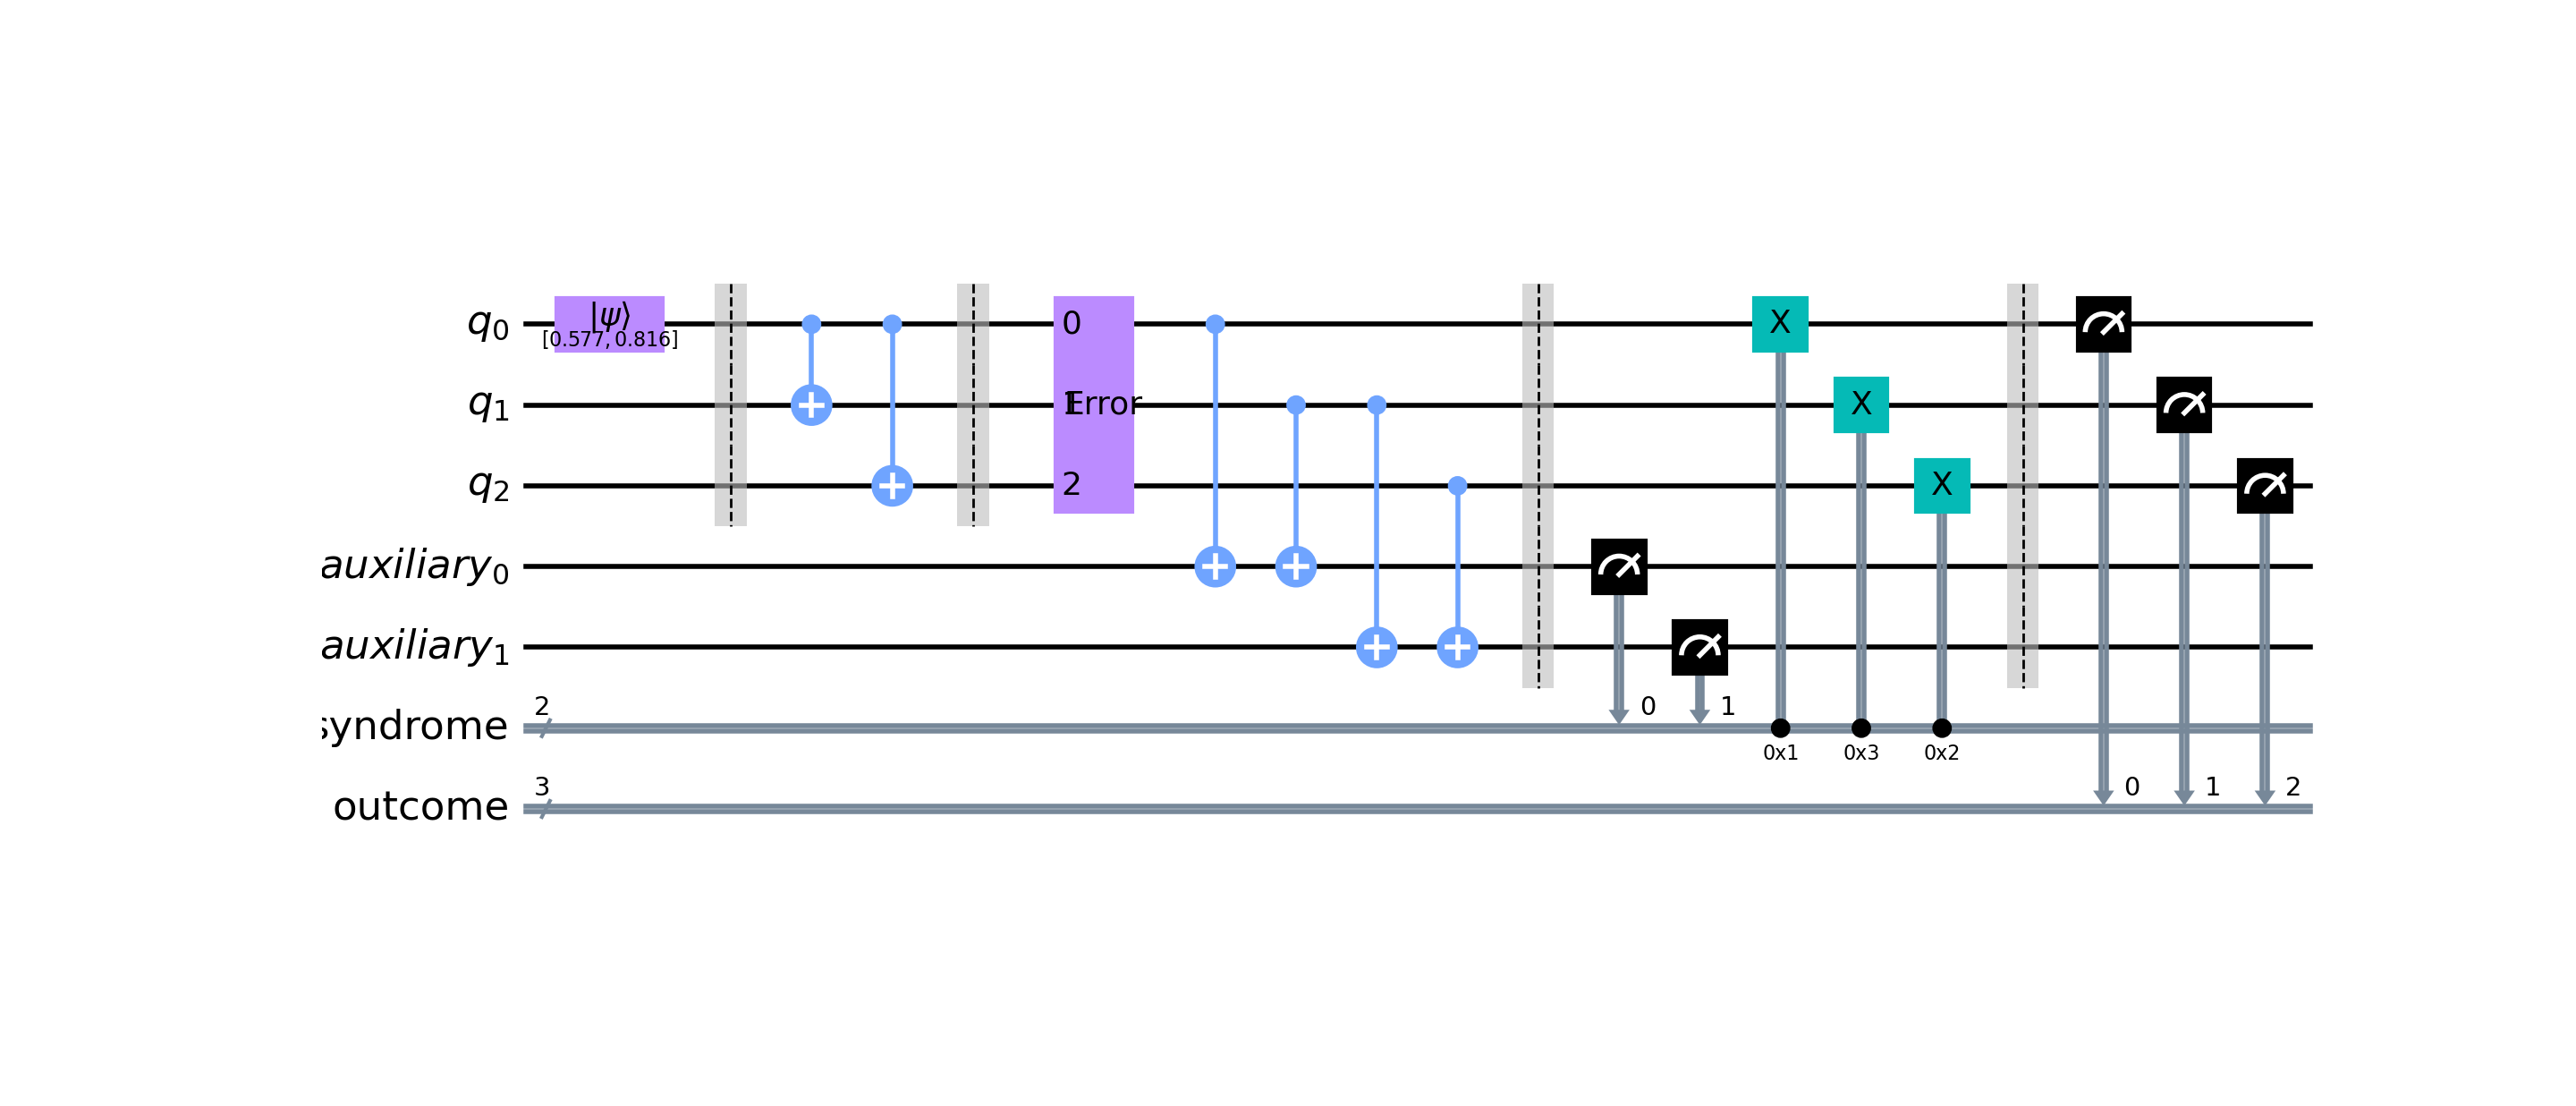
\includegraphics[width=\textwidth]{Mainmatter/images/3bitflipcode.png}
    \caption{Circuit for the 3 bit-flip error correction code, built with CNOT gates, which allows the correction of one X error on the encoded state. The M in the square represent a measurement on the ancilla qubits}
    \label{fig:3fq}
\end{figure}

The original information that we want to protect can be written without loss of generality as $\ket{\psi} = \alpha\ket{0}+\beta\ket{1}$.
As said in the previous section one might be tempted to clone the information like in the classical binary repetition code, but the no-cloning theorem prevents us from applying an operation that maps $\ket{\psi} \to \ket{\psi}\ket{\psi}\ket{\psi}$, showing that the classical idea cannot be directly taken over.
Instead, we can encode our qubit with other two qubits initially in the state $\ket{0}$. First we map the state $\ket{\psi} \to  \alpha\ket{000}+\beta\ket{100}$, then we apply two CNOT gates as shown in figure \ref{fig:3fq}, and encode the qubits in the following way: 
\begin{equation*}
  \alpha\ket{000}+\beta\ket{100} \to \alpha\ket{000}+\beta\ket{111} := \ket{\psi}_L
\end{equation*}
where we use the subscript $L$ to denote that the final encoded state lives in the logical two-dimensional subspace spanned by $\{\ket{0}_L = \ket{000} , \ket{1}_L = \ket{111}\}$ basis:
$$
|\psi\rangle_{L} \in \mathcal{C}=\operatorname{span}\{|000\rangle,|111\rangle\} \subset \mathcal{S}_{8}
$$
where $\mathcal{C}$ is called the codespace and its elements are the codewords.% We can also write the density operator that describe the system: $\rho=\ket{\psi_L}\bra{\psi_L}$.



Then the logical state $\ket{\psi}_L$ is sent down to the channel, and an error can occur. 


Notice that three individual bit flips are required to take $\ket{0}_L \leftrightarrow \ket{1}_L$, hence if we assume $\ket{\psi} = \ket{0}_L$, a single bit-flip on any qubit leaves the final state closer to $\ket{0}_L$ than $\ket{1}_L$. The distance between two codeword states, d, defines the number of errors that can be corrected, t, as, $t=\floor{\frac{d-1}{2}}$. In this case,d=3 because it is characterized by a weight $|\Tilde{X}|=|X_1 \otimes X_2 \otimes X_3 | = 3$ , hence $t=1$, but we will give a more in-depth explanation for the code distance and the number of correctable errors.



%The noise action on the qubits can be thought of as a set of Kraus operators which multiply the state of the system with some probabilities. We define an error set for the bit-flip noise: $\mathcal{E}=\left\{I,X^1,X^2,X^3\right\}$ as a set of operators proportional to Kraus operators. 
%The bit-flip noise acting on the qubit (i) can be written as: 
%\begin{equation*}
 %   \mathcal{E}^i(\rho) = (1-p)\rho +p X^i \rho X^i 
%\end{equation*}
%Generally, at least one of these operators (usually $\left.E_{0}\right)$ is taken to be the identity $I$ (at least to a good approximation), which corresponds to no error occurring, while the others represent possible errors. 
%Since the noise acts independently on each of the 3 qubits: 
%\begin{equation*}
 %   \mathcal{E}_{noise}(\rho)=\mathcal{E}^3(\mathcal{E}^2(\mathcal{E}^1(\rho)))
%\end{equation*} 
After the noisy channel the outcome state is one of the following:
\begin{equation*}
\begin{array}{ll}
\text { State } & \text { probability} \\
\alpha|000\rangle+\beta|111\rangle & (1-p)^{3} \\
\alpha|100\rangle+\beta|011\rangle & p(1-p)^{2} \\
\alpha|010\rangle+\beta|101\rangle & p(1-p)^{2} \\
\alpha|001\rangle+\beta|110\rangle & p(1-p)^{2} \\
% a|110\rangle+b|001\rangle & p^{2}(1-p) \\
% a|101\rangle+b|010\rangle & p^{2}(1-p) \\
% a|011\rangle+b|100\rangle & p^{2}(1-p) \\
% a|111\rangle+b|000\rangle & p^{3}
\end{array}
\end{equation*}
We get restricted on the case where only one physical qubit has been flipped, and ignore all the errors that flipped 2 or more qubits; in fact, the probability for this is of higher order $O(p^2)$ and the code will not be able to correct all of them.


Classically, single bit-flip errors are corrected by measuring the three bits and taking a majority vote. Here, this is not possible, since measuring the bits would project the system into one of the basis states with probability $|\alpha|^{2}$ or $|\beta|^{2}$,
destroying the superposition state that we are trying to protect. 

There is a two stage error-correction procedure which can be used to recover the correct quantum state without loosing the information: detect the error and correct it.  


In order to detect the error we have to do a measurement that reveals the error without revealing any information about the encoded state.
Error detection measurements are called syndrome measurements and the outcomes are called syndromes. 

In the quantum 3 bit-flip code one possible way to detect the error is to measure the correlation between two qubits, using two are commuting observables $Z_1 Z_2$ and $Z_2 Z_3$ with eigenvalues $\pm 1$.

%All four states are mutually orthogonal, hence they lie in orthogonal subspaces. Therefore, there is a quantum measurement that will tell which of these four subspaces the state is in without projecting onto a basis state and thereby destroying the superposition.

%We find that the outcomes of these syndrome measurements can detect and distinguish all single-qubit bit-flips, which can then be corrected. 


As shown in figure \ref{fig:3fq} this involves the use of two more qubits, these are called ancilla qubits.

The basic idea is to extract the syndrome performing two parity checks with the commuting observables $Z_1 Z_2$ and $Z_2 Z_3$ on the data block, and store the information in the ancilla qubits. 

Two initialized ancilla are then coupled to the data block as shown in figure \ref{fig:3fq}, using CNOT gates. 
We are left with 4 scenarios: 
\begin{equation*}
    \begin{array}{cc}
         \text{Error Location }& \text{Final State}, |data\rangle|ancilla\rangle \\
         \text{No Error} & (\alpha|000\rangle+\beta|111\rangle)|00\rangle \\
\text{Qubit 1} & (\alpha|100\rangle+\beta|011\rangle)|10\rangle \\
\text{Qubit 2} & (\alpha|010\rangle+\beta|101\rangle)|11\rangle \\
\text{Qubit 3} & (\alpha|001\rangle+\beta|110\rangle)|01\rangle 
    \end{array}
\end{equation*}
These ancilla are then measured. The measurement results indicate where (or if) an error has occurred, without directly measuring any of the data qubits.

In the end we use the value of the error syndrome to tell what procedure to use to recover the initial state:
\begin{equation*}
    \begin{array}{ccc}
        \text{Syndrome measurement:}
        (Z_1Z_2,Z_2Z_3) & \text{Ancilla state}& \text{Correction}\\
         (+1,+1) & |00\rangle & \text{Clean state, no correction needed }\\
(-1,+1) & |10\rangle & \text{Bit flip on qubit 1} \\
(-1,-1) & |11\rangle & \text{Bit flip on qubit 2}\\
(+1,-1) & |01\rangle  & \text{Bit flip on qubit 3}
    \end{array}
\end{equation*}

This bit-flip code has a correctable error set with four error operators: $\left\{I, X_{1}, X_{2}, X_{3}\right\}$. However, the full error set of this error model contained eight error operators. The three errors of weight- 2 and one error of weight-3 are uncorrectable errors. They produce states in the same four sub-spaces above, and it is easy to see that in the case of those high-weight errors the correction procedure will produce the erroneous state $\left|\psi_{L}^{\prime}\right\rangle=\alpha|111\rangle+\beta|000\rangle .$ In fact, the weight- 3 error will not even be recognized as an error: it is an undetectable error. This is a general property of QECCs: no QECC can correct every possible error. (This is also true of classical errorcorrecting codes.) In practice, the goal is to choose a code that can correct the most likely errors.

In analogous way of thinking, we can implement also the phase flip error code. In fact, a phase flip error in the computational basis ($\ket{0},\ket{1}$) can be seen as a bit flip in a new set of basis ($\ket{+},\ket{-}$), as shown in section \ref{sec:qgate}.

This suggests using the states $\ket{+},\ket{-}$ to create the logical encoded qubits: 
\begin{equation*}
    \begin{array}{c}
         \ket{0}_L=\ket{+++} \\
          \ket{1}_L=\ket{---}
    \end{array}
\end{equation*} these are the zero and the one states for protection against phase flip errors. 
To change basis in quantum circuit we can apply an Hadamard gate at appropriate points in the procedure.
The 3 phase-flip circuit is shown in figure \ref{fig:3phfc}

Then all the operations needed for error-correction are performed just as for the bit flip channel, but with respect to the new basis $\ket{+},\ket{-}$


We can improve our error analysis calculating the fidelity of this quantum error correction code, giving a measure of how reliable is this code against specific type of errors.
To calculate the fidelity is better to use the density matrix formalism, recalling the fact that the fidelity between a pure and a mixed state is given by :$ \mathcal{F}(\ket{\psi},\rho) = \bra{\psi}\rho\ket{\psi}$.
The object of quantum error-correction is to increase the fidelity with which quantum information is stored (or communicated) up near the maximum possible fidelity of one. Let’s compare the minimum fidelity achieved by the three qubit bit flip code with the fidelity when no error-correction is performed.
Suppose the quantum state of interest is $\ket{\psi}$ .
Without using the error-correcting code the state of the qubit after being sent through the channel is: 
\begin{equation*}
    \rho = (1-p)\ket{\psi}\bra{\psi} + p X\ket{\psi}\bra{\psi}X
\end{equation*}
Then the fidelity is given by
$$
F=\langle\psi|\rho| \psi\rangle=(1-p)+p\langle\psi|X| \psi\rangle\langle\psi|X| \psi\rangle
$$
The second term under the square root is non-negative, and equal to zero when $|\psi\rangle=|0\rangle$, so we see that the minimum fidelity is $F=1-p$ (No error correction code apply). Suppose the three qubit error correcting code is used to protect the state $|\psi\rangle=a\left|0_{L}\right\rangle+b\left|1_{L}\right\rangle.$ The quantum state after both the noise and error-correction is:
$$
\rho=\left[(1-p)^{3}+3 p(1-p)^{2}\right]|\psi\rangle\langle\psi|
$$
The omitted terms represent contributions from bit flips on two or three qubits. All the omitted terms are positive operators, so the fidelity we calculate will be a lower bound on the true fidelity. We see that $F=\langle\psi|\rho| \psi\rangle \geq (1-p)^{3}+3 p(1-p)^{2}$. That is, the fidelity is at least $1-3 p^{2}+2 p^{3}$, so the fidelity of storage for the quantum state is improved provided $p<1 / 2$.


\begin{figure}[h!]
    \centering
    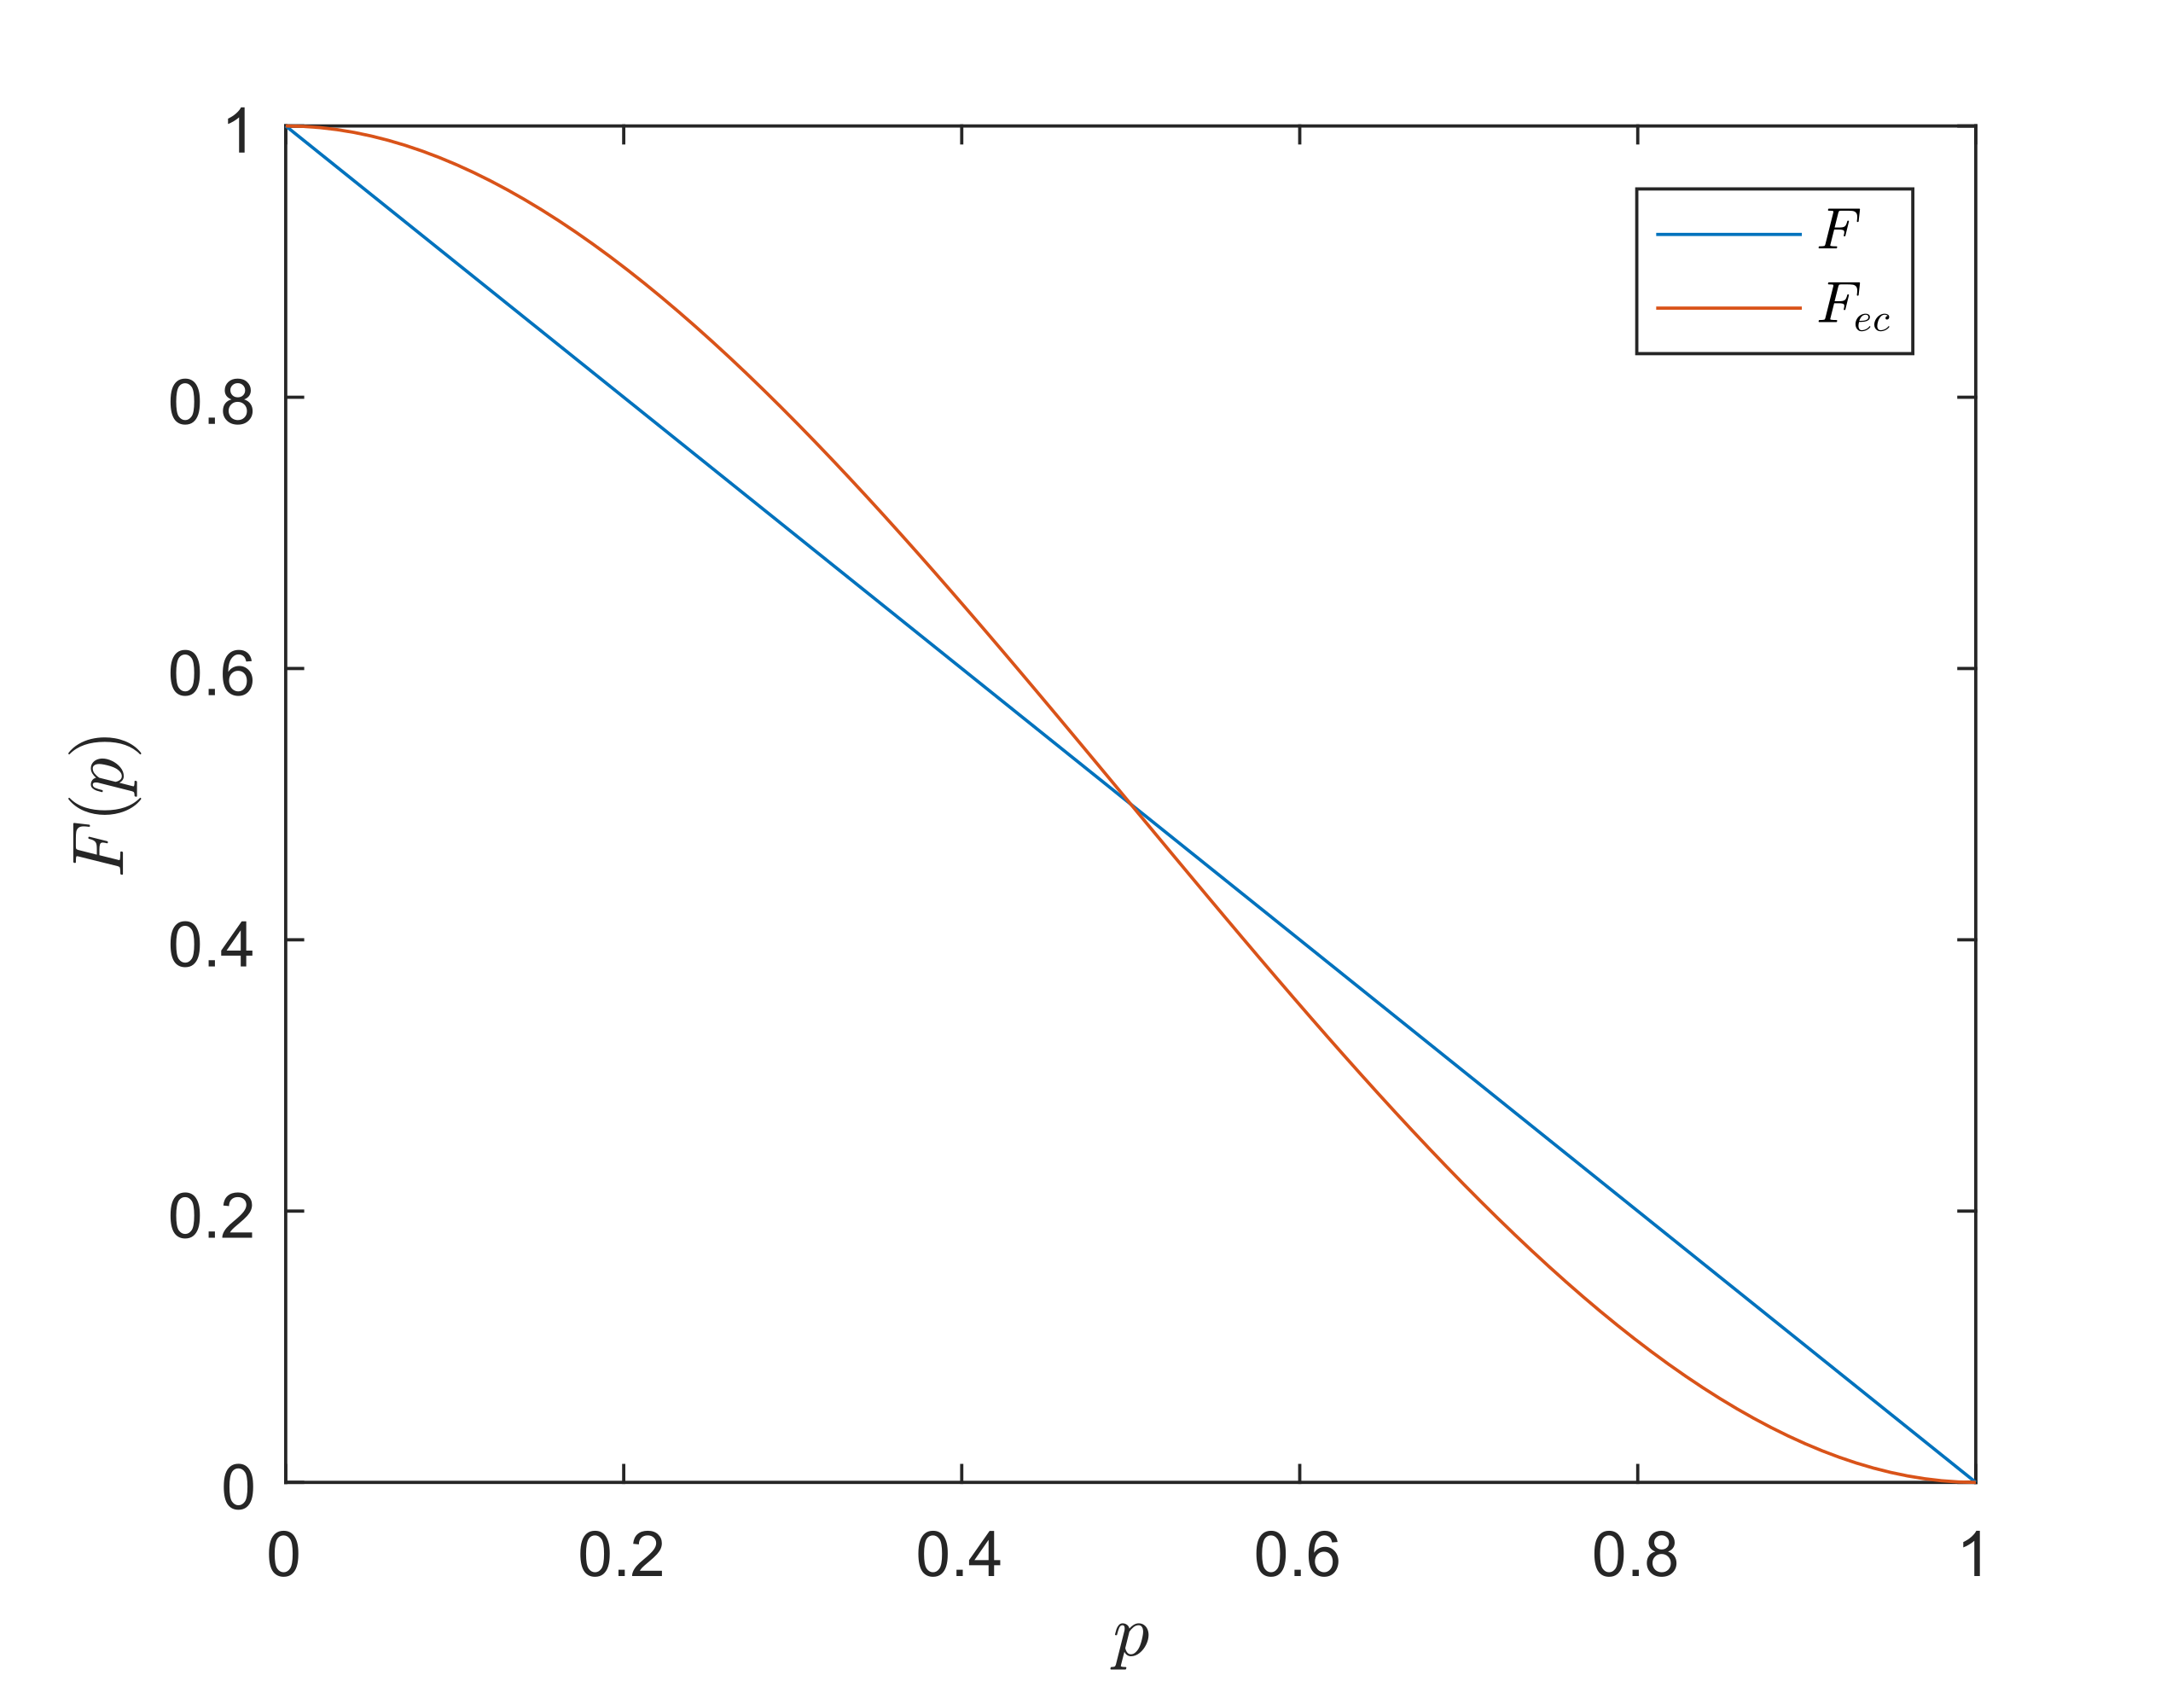
\includegraphics[scale=0.07]{Mainmatter/images/fidelity.png}
    \caption{In red the fidelity with the error correction procedure, in blue the fidelity without ( Currently this image is from wikipedia, but i will replace it with mine once I will do the computational part)}
    \label{fig:fidelity3qbit}
\end{figure}

\section{Stabilizer formalism}
In quantum error correction codes the description of quantum states becomes a difficult task when the number of qubits start rising, all the possible quantum states where the information can be projected by the noise grow exponentially in the number of qubits ($2^n$, where $n$ is the number of physical qubits). To understand complex quantum systems, it is essential to have efficient tools. The stabilizer formalism is a powerful tool that allows us to make general rules to construct preparation circuits, correction circuits and fault-tolerant logical gate operations once the stabilizer structure of the code is specified.


For example, the three-qubits code works by de-localising the information. The resultant logical state is then encoded in a two-dimensional subspace (the codespace $\mathcal{C}$) of the expanded Hilbert space. Then if an X-error occurs, the logical state is rotated to an orthogonal error space, an event that can be detected via a sequence of two stabilizer measurements and the result saved on some ancilla qubits, in the case of the three-qubit code the generators of the stabilizer group were $\{Z_1 Z_2 I, I Z_2 Z_3 \}$. 
%More in general the stabilizer formalism use the following scheme: 


%Usually a code is identified with this notation $[[n, k, d]]$ stabilizer codes, where $n$ is the total number of qubits, $k$ is the number of logical qubits and $d$ is the code distance. For instance the the three-qubit has $[[3,1,3]]$

%The advantage of entanglement-assisted stabilizer codes is that the sender can exploit the error-correcting properties of an arbitrary set of Pauli operators.

The definition of a stabilizer code is: 

Consider $\mathcal{S}=\{M\}$ to be a set of commuting error operators ($[M_i,M_j]=0 \quad \forall i,j$), this set is called Abelian. Since the operators all commute, they  have simultaneous eigenstates.
Let $\mathcal{C}=\{|u\rangle\}$ be an orthonormal set of simultaneous eigenstates all having eigenvalue $+1$:
\begin{equation}
M|u\rangle=|u\rangle \quad \forall u \in \mathcal{C}, \quad \forall M \in \mathcal{S}
\label{eq:stab}
\end{equation}
The set $\mathcal{C}$ is called codespace and its elements $|u\rangle$ are called code vectors or quantum codewords. 
A general state in the codespace is an encoded state or logical state, and it can be expressed as a superposition of the code vectors:
$$
|\psi\rangle_{L}=\sum_{u \in \mathcal{C}} a_{u}|u\rangle
$$ 
%Furthermore, $\mathcal{C}$ has $2^{k}$ members, since its members span a $2^{k}$ dimensional subspace of the $2^{n}$ dimensional Hilbert space of the whole system.
%On the other side, $\mathcal{S}$ is its stabilizer, its size is $2^{m}$, and it is spanned by $m =n-k$ linearly independent members of $\mathcal{S}$, where $n$ is the number of physical qubits and $k$ is the number of logical or encoded qubits.

%At this stage, the data previously stored solely in $\ket{\psi}$ is distributed across the expanded Hilbert space. 
A suitable stabilizer set of commuting operators acting on a single qubit can be a subgroup of the Pauli group:
$$
\mathcal{P}=\left\{\pm I, \pm i I, \pm X, \pm i X, \pm Y, \pm i Y, \pm Z, \pm i Z\right\}
$$

This set of matrices forms a group under the operation of matrix multiplication. The reason that the multiplicative factor $\pm 1 $ and $\pm i$ are included is to ensure that $\mathcal{P}$ is closed under multiplication, and thus forms a legitimate group. 
We can also generalize the concept of stabilizers for a system of multiple qubits. 
Given $n$ qubits a stabilizer set is a subgroup of the Pauli group $\mathcal{P}_n$, which is created by taking the $n$-fold tensor product of $\mathcal{P}$, i.e.
$$
\begin{aligned}
\mathcal{P}_{n} =\mathcal{P}^{\otimes n}
=\left\{\pm I, \pm i I, \pm X, \pm i X, \pm Y, \pm i Y, \pm Z, \pm i Z\right\}^{\otimes n}
\end{aligned}
$$

We can now define stabilizers more precisely: a subgroup $\mathcal{S} \subseteq \mathcal{P}_{n}$ is called stabilizer group of a system of $n$ qubits with $k$ logical qubits, and $\mathcal{C}$ is the vector space stabilized by $\mathcal{S}$.  

One feature of the stabilizer codes is that we can start from a stabilizer set and then deduct a codeword.
A perfect example, (again), is the three-qubit code ($n=3$), then start defining a stabilizer set $\mathcal{S} \equiv \{III,Z_1Z_2I,$ $IZ_2Z_3,Z_1IZ_3\}$. 
The subspace fixed by the operator $Z_1Z_2I$ is spanned by $|000\rangle$, $|001\rangle,|110\rangle$ and $|111\rangle$, and the subspace fixed by $IZ_{2} Z_{3}$ is spanned by $|000\rangle,|100\rangle,|011\rangle$ and $|111\rangle$. 
Note that the elements $|000\rangle$ and $|111\rangle$ are common to both these lists. Consequently, $\mathcal{C}$ must be the sub-space spanned by the states $|000\rangle$ and $|111\rangle$. 
Looking at this example we noticed that the sub-spaces have been stabilized by only two of the operators in $\mathcal{S}$.
In fact, mathematically a group can be described by its generators.
A set of elements $\{g1,...,gl\}$ in a group $G$ is said to generate the group $G$ if every element of $G$ can be written as a product of some of its elements. In the example $\mathcal{S}= \langle Z_1Z_2I,IZ_2Z_3\rangle$ as $Z_1IZ_3 = (Z_1Z_2I)(IZ_2Z_3)$ and $III = (Z_1Z_2I)^2$.
The great advantage of using generators to describe groups is that they provide a compact means of describing the group.
Nevertheless, not just any subgroup $\mathcal{S}$ of the Pauli group can be used as the stabilizer for a nontrivial vector space. For example, consider the subgroup of $\mathcal{P}_{1}$ consisting of $\{\pm I, \pm X\}$, the only solution to $(-I)|\psi\rangle=|\psi\rangle$ is $|\psi\rangle=0$, and thus $\{\pm I, \pm X\}$ is the stabilizer for the vector space with only the null vector. Hence, Two conditions are necessary in order not to span a trivial vector space :
\begin{enumerate}
    \item the stabilizer subgroup is Abelian ( i.e the elements of $\mathcal{S}$ commute)
    \item $-I$ and $-iI$ are not an element of the stabilizer set.
\end{enumerate}  

The definitions of stabilizer group and the codespace are of principal interest in QEC. 
One can show that if a stabilizer group $\mathcal{S}$ has $n-k$ independent generators, then $\operatorname{dim}[\mathcal{S}]=2^{n-k}$ and $\operatorname{dim}\left[\mathcal{C}\right]=2^{k}$, where $n$ indicates the number of physical qubits utilized and $k$ the logical qubits represented. %citare il libro
Whenever possible, $\mathcal{S}$ is typically represented through its independent generators $\mathcal{S}=<g_{1}, g_{2}, \ldots, g_{n-k}>$.





To understand how stabilizer codes detect and correct errors it is helpful to assume that the set of errors also consists of operators from the Pauli group. 

Each code allows correction of a particular set $\mathcal{E}=\{E\}$ of correctable errors.

Suppose that an error operator $E$ (which is also an element of the Pauli group) acts on the state. It anticommutes with some of the stabilizer generators, and commutes with others.
\begin{equation}
    M(E\ket{\psi}_L) = \pm EM\ket{\psi}_L = \pm (E\ket{\psi}_L)
    \label{eq:stabcond}
\end{equation}

Multiplying by $E$ changes the codeword to a new eigenstate of the stabilizer generators, where the eigenvalue is still $+1$ for all the generators that commute with $E$, but is $-1$ for those generators that anticommute with $E$.

%The eigenvalue of an operator $M$ from the stabilizer set detects errors which anticommute with $M$.
%On the contrary, if 
The measured eigenvalues $\lambda=\pm 1$ for each generator are the error syndrome.
To extract the syndrome we measure all the observables in the stabilizer. To do this, it is sufficient to measure any set of $n-k$ linearly independent $M$ in $\mathcal{S}$. Note that such a measurement has no effect on a state in the encoded subspace, since it is already an eigenstate of all these observables. The measurement projects a noisy state onto an eigenstate of each $M$, with eigenvalue $\lambda=\pm 1$.
The error can be deduced from the syndrome, hence to detect which error affected our logical qubit we need to store the results from the syndrome measurements. 

The syndrome extraction can be done most simply by attaching an $n-k$ qubit ancilla $A$ to the system, and storing in it the eigenvalues by a sequence of CNOT gates and Hadamard rotations.

The eigenvalue extraction of operator $M$, is done by preparing an ancilla in $(|0\rangle+|1\rangle) / \sqrt{2}$. 
Then, operate controlled-$M$ with ancilla as control, and system as target, then apply an Hadamard rotations to the ancilla. 
The final state of the ancilla is:  $[(1+\lambda)|0\rangle+(1-\lambda)|1\rangle] / 2$. In other words, if the stabilizer commute with the error operation ($\lambda=+1$) the ancilla final state will be $\ket{0}$, and viceversa. The syndrome measurements given by the application of the stabilizers are stored in the ancilla states. Repeating this process for all the $n-k$ operators $M$ which span $\mathcal{S}$, the effect is to couple system with the ancilla as follow:
$$
|0\rangle_{a} \sum_{i}\left(E_{i}|\phi\rangle_{L}\right) \rightarrow \sum_{i}\left|s_{i}\right\rangle_{a}\left(E_{i}|\phi\rangle_{L}\right)
$$
The syndromes $s_{i}$ are $(n-k)$ -bit binary strings. So far the treatment is completely general.
Now suppose the $E_{i}$ all have different syndromes. Then a projective measurement of the ancilla will collapse the sum to a single term taken at random: $\left|s_{i}\right\rangle_{a}\left(E_{i}|\phi\rangle_{L}\right)$, and will yield $s_{i}$ as the measurement result. 
The measurement result of the ancilla determines which eigenstate $\ket{\psi}_L$ is projected into.
Since there is only one $E_{i}$ with this syndrome, we can deduce the operator $E_{i}$ and correct it. 

This is the general prescription for correcting errors with a stabilizer code. One measures the values ±1 of the stabilizer generators; from the resulting error syndrome, one deduces which error occurred, and correct it(which for Pauli operators means just applying the error again). If the true error operator was actually a linear combination of Pauli operators, measuring the stabilizer generators will project the state into a joint eigenspace, and one proceeds exactly as if the error had been a Pauli operator. Just like linear codes, for a small stabilizer code one can use a look-up table of error syndromes; for a larger code, a decoding algorithm is needed.
% The exact network is shown in figure \ref{fig:stab}
% \begin{figure}[h!]
%     \centering
%     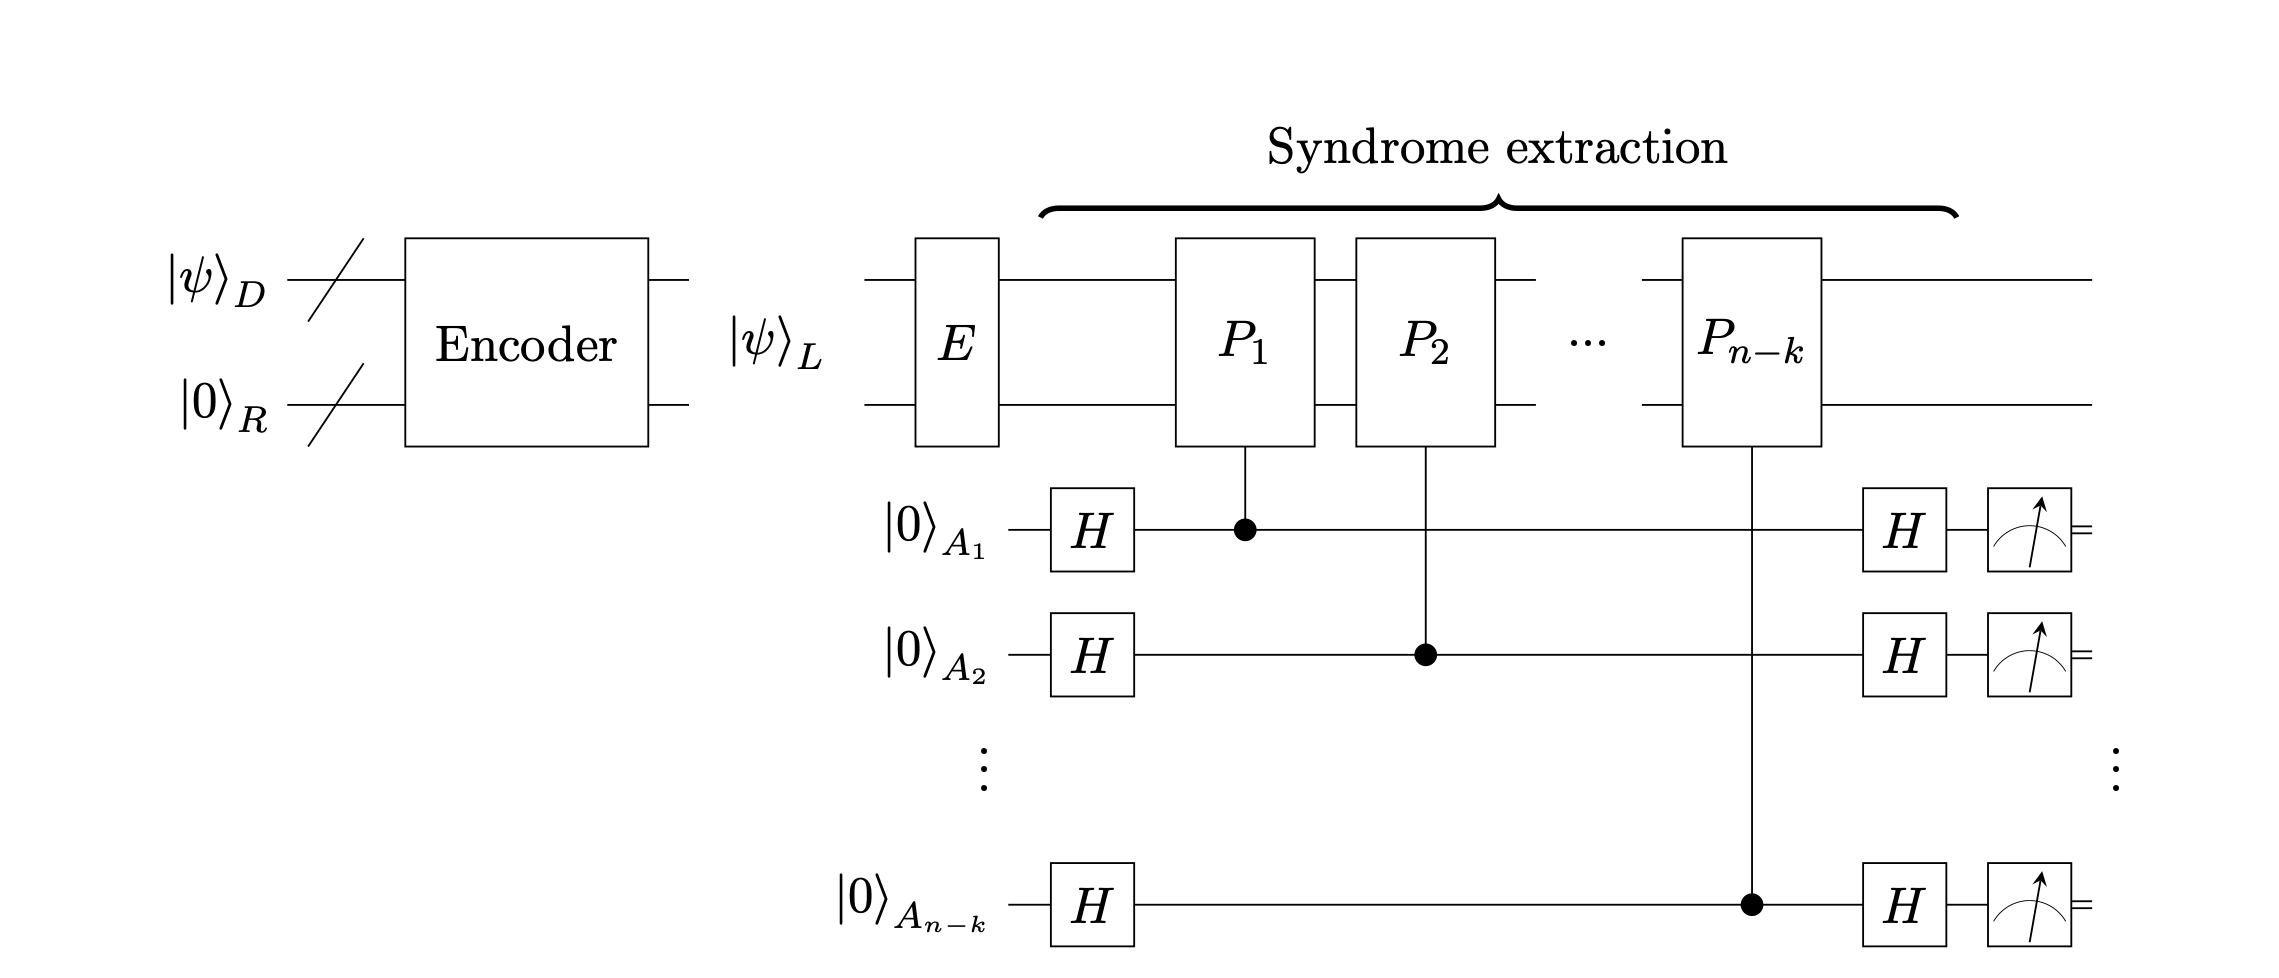
\includegraphics[width=\textwidth]{Mainmatter/images/Sindromeextraction.png}
%     \caption{}
%     \label{fig:stab}
% \end{figure}


Let us see how this works for the bit-flip code. It has generators $g_{1}=Z Z I$ and $g_{2}=I Z Z$. The three weight-one errors are $E_{1}=X I I, E_{2}=I X I, E_{3}=I I X .$ We can see that $E_{1}$ anticommutes with $g_{1}$ and commutes with $g_{2} ; E_{2}$ anticommutes with both $g_{1}$ and $g_{2}$; and $E_{3}$ anticommutes with $g_{2}$ and commutes with $g_{1}$. Since $g_{1}$ and $g_{2}$ are commuting observables, we can measure them to diagnose which error happened (or no error). The measured values $\pm 1$ for each generator are the error syndrome. Since Pauli operators are unitary and square to the identity, we can then undo the effects of the error by applying the appropriate Pauli operator again.

\section{Quantum code distance}
A quantum correction code can be identified by 3 parameters using the following notation: $[[n, k, d]]$\footnote{The doublebrackets are used simply to denote that the code being referred to is a quantum error correction code rather than a classical code.}. This means that a QECC encodes $k$ logical qubits using $n$ physical qubits , in such a way that any operation which maps some encoded state to another encoded state must act on at least $d$ qubits. 
So far we saw the physical and encoded qubits, but we never focused on the third parameter, so let's define what it is the code distance better, using the stabilizer formalism. 
As shown in the previous chapters, the eigenvalue of an operator $M \in \mathcal{S}$ from the stabilizer detects errors which anticommute with $M$.
On the other hand, if any of those errors which commute with $M$ occurs, the code it is not be able to detects the error anymore. This is because if we measure the eigenvalue of all the generators of the stabilizer they are all still $+1$, and also the correct codeword has eigenvalue $+1$ so there is no way that we can tell if any error occurs. In fact, stabilizer maps codewords in codewords, it is not that we don't measure the right thing actually there is no way to tell. 

In particular let's define a stabilizer set $\mathcal{S}$, and let $\mathrm{T}(\mathrm{S})$ be the corresponding QECC.
Define then,
$$
N(S)=\left\{N \in P_{n} \text { s.t. } M N=N M \forall M \in S\right\}
$$
and errors in this space are undetectable errors. 
Hence, we can say that a general QECC detects any error not in $\mathrm{N}(\mathrm{S}) \backslash \mathrm{S}$ (i.e., errors which commute with the stabilizer are not detected). We need also to remove all the error in $S$ because "errors" in S leave all codewords fixed, so are not really errors (Degenerate QECC, like the Shor code)
In this way, we are left with all those errors which anticommute with some M and can be detected. Starting from this point we can define the distance d. 
The distance d of $\mathrm{T}(\mathrm{S})$ is the weight of the smallest Pauli operator $\mathrm{N}$ in $\mathrm{N}(\mathrm{S}) \backslash \mathrm{S}$.

Intuitively, this can be though as the number of qubit that we need to flip to obtain another codeword. In other words, as is the case for classical codes, the distance of a quantum code is defined as the minimum size error that will go undetected.

This definition of distance tells us not only which errors can be detected but also how many of them can we correct. 
We can tell how many errors the code corrects by looking at operators that commute with the stabilizer. 



We say that a QECC can correct t errors if the set of errors that allow the recovery (those errors not in $\mathrm{N}(\mathrm{S}) \backslash S$) of weight t or less, must satisfy the sufficient conditions for the code to be able to correct the error: 
\begin{equation*}
    \bra{i} E_a^{\dagger}E_b \ket{j} = C_{a,b}\delta_{ij}
\end{equation*}
where $E_a^{\dagger}E_b \notin \mathrm{N}(\mathrm{S}) \backslash S$, and the states $i$ and $j$ are codewords.
%by  $E$ and $F$ if either $E^{\dagger} F \in S$ (so $E$ and $F$ act the same on codewords), or if $\exists M \in S$ s.t. $\left\{M, E^{\dagger} F\right\}=0$, in which case measuring the operator $M$ distinguishes between $E$ and $F$.
%The code correct errors for which $E^{\dagger}F \notin N(S) \backslash S$ for all possible pairs of errors E and F. 

Therefore, to correct t errors, we should look to all these pairs $E_a^\dagger E_b$ that show up in the criterion. Each $E_{a,b}$ acts on t qubit (correspondingly to the weight), but $E_a^\dagger E_b$ acts on $2t$ qubits. Then, the smallest thing in $N(S)\backslash S$ should be at least of weight $2t +1$. 


To sum up, if we want to correct error with  weight t, we need a code distance $d \ge 2t+1$.
Let's take a fast example, (again), the bit-flip code. 
In this code the smallest operator that transform $\ket{0}_L$ to $\ket{1}_L$, or vice versa, it
is $\Bar{X}=X_1X_2X_3$. 
If it were the case that qubits were only susceptible to $X-errors$, then the three-qubit code would have distance $d = 3$, cause each pauli operator has weight $1$
and to obtain another codeword you need 3 of them. 
However, as qubits are also susceptible to phase-flip errors like Z errors. The action of Z maps a codeword to another one, hence, for the bit-flip code a Z error is undetectable. Hence the real distance for this code is $d=1$. 
% In other words, this minimum size error can be viewed as a logical Pauli operator that transforms one codeword state to another. 



% This new eigenstate will always be orthogonal to the original codeword unless the error operator commutes with all the stabilizer generators.
%(So, for example, any encoded state which has been subjected to an error consisting of at most $\lfloor(d-1) / 2\rfloor$ Pauli operations can in principle be recovered perfectly).
%This notation generalises the notation $[n, k, d]$ for classical error correction codes. %in such a way that at least $d$ bits must be flipped to transform between any two codewords representing different plaintexts. (In this context and in the quantum case, $d$ is referred to as the code distance.) 
%
%The distance is the smallest size of a detectable error




\section{Shor code, $[[9,1,3]]$}
The Shor code is an example of a distance-three degenerate code for which it is possible to apply a successful recovery operation for any single-qubit error. This code uses 9-qubits, and it was the first QECCs that was capable of correcting any arbitrary error (Phase and bit flip) on a single qubit, protecting one logical qubit state.
The Shor code can be constructed by concatenating the bit-flip code and the phase-flip code. 
Code concatenation involves embedding the output of one code into the input of another.
So let's start building the encoded Shor states from the codespace of the bit-flip and the phase-flip code. 

Consider the codespace of a single bit-flip code: 
$$
\mathcal{C}_{3b}=\operatorname{span}\left\{|0\rangle_{3b}=|000\rangle,|1\rangle_{3 b}=|111\rangle\right\}, \quad \mathcal{S}_{3 b}=\left\langle Z_{1} Z_{2}, Z_{2} Z_{3}\right\rangle
$$
where $\mathcal{S}_{3b}$ are the code stabilizers. Similarly, codespace for phase-flips $\mathcal{C}_{3 \mathrm{p}}$ is defined
$$
\mathcal{C}_{3 \mathrm{p}}=\operatorname{span}\left\{|0\rangle_{3 \mathrm{p}}=|+++\rangle,|1\rangle_{3 \mathrm{p}}=|---\rangle\right\}, \quad \mathcal{S}_{3 \mathrm{p}}=\left\langle X_{1} X_{2}, X_{2} X_{3}\right\rangle
$$
Then to build the nine-qubit code, the bit-flip code is embedded into the codewords of the phase-flip code. This concatenation maps the $|0\rangle_{3 \mathrm{p}}$ codeword of the phase-flip code to a nine-qubit codeword $|0\rangle_{9}$ as follows
$$
|0\rangle_{3 \mathrm{p}}=|+++\rangle \stackrel{\text { concatenation }}{\longrightarrow}|0\rangle_{9}=|+\rangle_{3 \mathrm{b}}|+\rangle_{3 \mathrm{b}}|+\rangle_{3 \mathrm{b}}
$$
where $|+\rangle_{3 \mathrm{~b}}=\frac{1}{\sqrt{2}}(|000\rangle+|111\rangle)$ is a logical state of the bit-flip code. 

Similarly, the concatenation maps the $|1\rangle_{3 \mathrm{p}}$ codeword of the phase-flip code to
$$
|1\rangle_{3 \mathrm{p}}=|---\rangle \stackrel{\text { concatenation }}{\longrightarrow}|1\rangle_{9}=|-\rangle_{3 \mathrm{~b}}|-\rangle_{3 \mathrm{~b}}|-\rangle_{3 \mathrm{~b}},
$$
where $|-\rangle_{3b}=\frac{1}{\sqrt{\Omega}}(|000\rangle-|111\rangle)$. The code defined by the codewords $|0\rangle_{9}$ and $|1\rangle_{9}$ is the nine-qubit Shor code with paramaters $[[9, 1, 3]]$


Finally, the qubit state (the sending information) $|\psi\rangle=\alpha|0\rangle+\beta|1\rangle$ is encoded as $\left|\psi_{L}\right\rangle=\alpha\left|0_{L}\right\rangle+\beta\left|1_{L}\right\rangle$. Hence the codespace basis is: 
\begin{equation*}
\begin{split}
\left|0_{L}\right\rangle=\frac{1}{2 \sqrt{2}}(|000\rangle +|111\rangle) \otimes(|000\rangle +|111\rangle) \otimes(|000\rangle +|111\rangle) \\
\left|1_{L}\right\rangle=\frac{1}{2 \sqrt{2}}(|000\rangle -|111\rangle) \otimes(|000\rangle -|111\rangle) \otimes(|000\rangle -|111\rangle) 
\end{split}
\end{equation*}

Once one has find the codespace, it can also can look for a stabilizer set. Since this code is a concatenation of the bit-flip code and the phase-flip code one might use the same stabilizers but with more accuracy. 
A suitable stabilizer set is spanned by: 
\begin{equation}
\begin{aligned}
\mathcal{S}_{[[9,3,3]]}=&\left\langle Z_{1} Z_{2}, Z_{2} Z_{3}, Z_{4} Z_{5}, Z_{5} Z_{6}, Z_{7} Z_{8}, Z_{8} Z_{9}\right.\\
&\left.X_{1} X_{2} X_{3} X_{4} X_{5} X_{6}, X_{4} X_{5} X_{6} X_{7} X_{8} X_{9}\right\rangle
\end{aligned}
\end{equation}

The first six terms are the stabilizers of the bit-flip codes in the three-blocks of the code. The final two stabilizers derive from the stabilizers of the phase-flip code.

Hence, using the stabiliser formalism we can proceed for the syndrome measurement. 
\begin{table}[h]
    \centering
    \begin{tabular}{cc|cc}
\hline Error & Syndrome, $S$ & Error & Syndrome, $S$ \\
\hline$X_{1}$ & 10000000 & $Z_{1}$ & 00000010 \\
$X_{2}$ & 11000000 & $Z_{2}$ & 00000010 \\
$X_{3}$ & 01000000 & $Z_{3}$ & 00000010 \\
$X_{4}$ & 00100000 & $Z_{4}$ & 00000011 \\
$X_{5}$ & 00110000 & $Z_{5}$ & 00000011 \\
$X_{6}$ & 00010000 & $Z_{6}$ & 00000011 \\
$X_{7}$ & 00001000 & $Z_{7}$ & 00000001 \\
$X_{8}$ & 00001100 & $Z_{8}$ & 00000001 \\
$X_{9}$ & 00000100 & $Z_{9}$ & 00000001 \\
\hline
\end{tabular}
\caption{The syndrome table for single-qubit $X$ and $Z$ errors on the nine-qubit code. The nine-qubit code is a degenerate code, as certain $Z$ errors share the same syndrome}
    \label{tab:stab9}
\end{table}

Table \ref{tab:stab9} shows the syndromes for all single-qubit errors in the nine-qubit code. Each of the $X$ errors produce unique syndromes. In contrast, $Z$ -errors that occur in the same block of the code have the same syndrome. Fortunately, this degeneracy in the code syndromes does not reduce the code distance. To see why this is the case, consider the single-qubit errors $Z_{1}$ and $Z_{2}$, both of which map to the syndrome '00000010'. The decoder therefore has insufficient information to differentiate between the two errors, and will output the same recovery operation for either. For the purposes of this example, we will assume that the recovery operation the decoder outputs is $\mathcal{R}=Z_{1}$. For the case where the error is $E=Z_{1}$, the recovery operation restores the logical state as $\mathcal{R} E|\psi\rangle_{9}=Z_{1} Z_{1}|\psi\rangle_{9}=|\psi\rangle_{9} .$ In the event where $E=Z_{2}$, the recovery operation still restores the logical state as $\mathcal{R} E=Z_{1} Z_{2}$ is in the stabilizer of $\mathcal{C}_{[[9,1,3]]}$, and therefore acts on the logical state as follows $Z_{1} Z_{2}|\psi\rangle_{9}=|\psi\rangle_{9} .$ The same arguments can be applied to the remaining degenerate errors of the code. As a result, the nine-qubit code has the ability to correct all single-qubit errors and has distance $d=3$
In this code the process of correcting a X error or a Z error is totally independent: 
the inner layer of the code corrects bit flip errors taking the majority within each set of three, so 
On the other hand, the outer layer corrects phase flip errors: We take the majority of the three signs,
Since these two error correction steps are independent, the code also works if there is both a bit flip error and a phase flip error, and since $Y = iZX$, a $Y$ error can be thought as a single $X$ error and a single $Z$ error acting on the same qubit, up to an irrelevant global phase.

So this code can correct any Pauli error acting on a single qubit. However, even this is not the limit. Note that any operator on a single qubit can be written as a linear combination $E= aI + bX + cY+dZ$ for some complex numbers $a,b,c,d$. This allow us, using this code, to correct also a continuous tipe of errors. For instance, suppose the action of a general phase error on the codeword: 
$$
R_{\theta / 2}=\left(\begin{array}{cc}
1 & 0 \\
0 & e^{i \theta}
\end{array}\right)=e^{i \theta / 2}\left(\begin{array}{cc}
e^{-i \theta / 2} & 0 \\
0 & e^{i \theta / 2}
\end{array}\right)
$$
(with an overall phase that does not matter), we can write it as
$$
R_{\theta / 2}=\cos \frac{\theta}{2} I-i \sin \frac{\theta}{2} Z .
$$
It turns out that our earlier error correction procedure will also correct this error.
This can suggest a bigger result expressed by the following theorem [3]:

\begin{theorem}
If a quantum code corrects errors A and B, it also corrects any linear combination of A and B. In particular, if it corrects all weight t Pauli errors, then the code corrects all t-qubit errors.
\end{theorem}


\section{CSS codes}
CSS codes are a very special class of stabilizer codes with special properties. In fact, principles from the theory of classical error correction codes can be adapted for the construction of quantum error correction codes. Those quantum error correction codes can be driven from the classical codes and are called CSS codes.
Before introducing a CSS code construction, is better to do a brief recall of classical error correction codes, and we will take the Hamming code as a landmark.
There are two ways of representing a classical linear code and find its codewords: either as the image of a matrix G called the generator matrix or as the kernel of matrix H called the parity check matrix. More precisely we can define a linear classical error correcting code $\mathcal{C}$ of n-bit vectors by: $x \in \mathcal{C} \iff  Hx = 0$ with the linear property: $x,y \in \mathcal{C} \rightarrow x+y \in \mathcal{C}$. Moreover, $HG^T=0$ because each row of the generator matrix is a codeword and must satisfy the parity check; the other codewords are all linear combinations of the rows of the generator matrix.
%Another important definition is the dual code $\mathcal{C}^{\perp}$ of a linear code $\mathcal{C}$, this is the code whose generator matrix is the parity check matrix of $\mathcal{C}$. 
We can deduce a similarity between the parity check matrix and the stabilizer set. 
In fact, in classical codes if an error occur it affects the codeword as follow $x+e_1$ , and no longer satisfy the parity check $H(x+e_1) = He_1 \neq 0$. An analogous situation corresponds when an error occurs and the condition (\ref{}) is no longer satisfied.  
Hence, we can see the rows of H as indicators of which stabilizers are needed.
A well known classical correcting code is the Hamming code which is [7,4,3]. The parity check of this code is: 
\begin{equation*}
    H=\left(\begin{array}{ccccccc}
         1&1&1&1&0&0&0  \\
         1&1&0&0&1&1&0 \\
         1&0&1&0&1&0&1 
    \end{array}\right) 
\end{equation*}
If we replace each 1 in this matrix by the operator Z, and 0 by I, we are just specifying three operators that implement the parity check measurements. The statement that the classical Hamming code corrects one error is the statement that each bit flip error of weight one or two anticommutes with one of these three operators.
\begin{equation*}
    H_1=\left(\begin{array}{ccccccc}
         1&1&1&1&0&0&0  \\
         1&1&0&0&1&1&0 \\
         1&0&1&0&1&0&1 
    \end{array}\right) \to \mathcal{S}_{bf}=\left\langle\begin{array}{ccccccc}
         Z&Z&Z&Z&I&I&I  \\
         Z&Z&I&I&Z&Z&I \\
         Z&I&Z&I&Z&I&Z 
    \end{array}\right\rangle
\end{equation*}
However, qubits are subjected to phase-flips as well. We can use again the same procedure; we replace each 1 by X instead of Z and we can correct a phase error. We again get three operators, and they will anticommute with any weight one or two Z error.
\begin{equation*}
    H_2=\left(\begin{array}{ccccccc}
         1&1&1&1&0&0&0  \\
         1&1&0&0&1&1&0 \\
         1&0&1&0&1&0&1 
    \end{array}\right) \to \mathcal{S}_{pf}=\left\langle\begin{array}{ccccccc}
         X&X&X&X&I&I&I  \\
         X&X&I&I&X&X&I \\
         X&I&X&I&X&I&X 
    \end{array}\right\rangle
\end{equation*}
Thus, if we make a stabilizer out of the three Z operators and the three X operators, we get a code that can correct any single qubit error. X errors are picked up by the first three generators, Z errors by the last three, and Y errors are distinguished by showing up in both halves. 
\begin{equation}
    \mathcal{S} : \begin{array}{ccccccc}
         Z&Z&Z&Z&I&I&I  \\
         Z&Z&0&I&Z&Z&I \\
         Z&I&Z&I&Z&I&Z \\
         X&X&X&X&I&I&I  \\
         X&X&I&I&X&X&I \\
         X&I&X&I&X&I&X 
         \end{array}
         \label{eq:stabSteane}
\end{equation}
We solved a difficult problem as finding a stabilizer set of a quantum error correcting code with a minimum effort using the knowledge from the classical theory.
But there is one thing that we need to pay attention when we use this procedure: the stabilizer must be Abelian, i.e. all the elements commute.
In the previous example, the stabilizer set is Abelian and the corresponded code is the Steane code $[[7,1,3]]$.
 
This example uses the same classical code for both the $X$ and $Z$ generators, but there was no reason to do so. We could have used any two classical codes $C_{1}$ and $C_{2}$. The only requirement is that the $X$ and $Z$ generators commute. This corresponds to the statement that $C_{2}^{\perp} \subseteq C_{1}\left(C_{2}^{\perp}\right)$ is the dual code to $C_{2}$\footnote{$C_2^{\perp}$ is the dual code of $C_2$, intuitively this means that in $C_2^{\perp}$ the generator matrix and the parity matrix are switched respect $C_2$. In other words it consists  of those words which are orthogonal to the codewords of $C_{2}$)}.
If $C_{1}$ is an $\left[n, k_{1}, d_{1}\right]$ code, and $C_{2}$ is an $\left[n, k_{2}, d_{2}\right]$ code, then the corresponding quantum code is an $\left[\left[n, k_{1}+k_{2}-n, \min \left(d_{1}, d_{2}\right)\right]\right]$ code. 

   %have a particularly nice form. One way to write down the quantum codewords is:
% $$
% |u\rangle_{L}=\frac{1}{\sqrt{dim(C_2^{\perp})}}\sum_{x \in C_{2}^{\perp}}|x+u \cdot D\rangle
% $$
% where $u$ is a $k$ -bit binary word, $x$ is an $n$ -bit binary word, and $D$ is a $(k \times n)$ matrix of coset leaders. A coset leader is a word of minimum weight in any particular coset, which is a word with the lowest amount of non-zero entries We can understand the structure of these codewords as follows. 
% Start with the case $u=0: |0\rangle_{L}$ is an equal superposition of all the members of $C_{2}^{\perp}.$ 
% The next encoded state is found by displacing all the members of $C_{2}^{\perp}$ by the same vector (the first row of $\left.D\right)$ : in other words we have a superposition of all the members of a coset. We choose the vector (the coset leader) so that this coset is still in $C_{1}$. The other quantum codewords are formed similarly by further cosets of $C_{2}^{\perp}$, all within $C_{1}$. Bit flip correction follows from the%They all must satisfy the same parity checks as the classical code $C_{1}$, so all codewords will be superpositions of codewords of $C_{1} .$ The parity check matrix of $C_{2}$ is the generator matrix of $C_{2}^{\perp}$, so the $X$ generators of the stabilizer add a word of $C_{2}^{\perp}$ to the state. Thus, the codewords of a CSS code are of the form
% $$
% \sum_{w \in C_{2}^{\perp}}|u+w\rangle
% $$
% where $u \in C_{1}\left(C_{2}^{\perp} \subseteq C_{1}\right.$, so $\left.u+w \in C_{1}\right) .$

%The basis of the quantum code 
The codewords of a CSS code, in this case the Steane code, include two entangled states obtained from the classic codewords of each coset of $\mathrm{C}_1$ relative to $\mathrm{C}_2^{\perp}:$ the logical 0 is given from all the codewords with even weight $\mathrm{C}_2^{\perp} \oplus(0000000)$:
% and the $\mathrm{C}^{\perp} \oplus(1111111)=\{$ codewords of $\mathrm{C}$ with odd weight $\}$. The quantum codewords are:

$$
\begin{array}{r}
\left|0\right\rangle_L=\frac{1}{\sqrt{8}}[|0000000\rangle+|1010101\rangle+|0110011\rangle+|1100110\rangle \\
+|0001111\rangle+|1011010\rangle+|0111100\rangle+|1101001\rangle]
\end{array}
$$
To determine the other logical codeword we need to find an element of $C_{1}$ that is not in $C^{\perp}_{2}$. An example of such an element is $(1111111)$, giving then the other logical qubit, which this time is formed by all the codewords with odd weight:
$$
\begin{array}{r}
\left|1\right\rangle_L=\frac{1}{\sqrt{8}}[|1111111\rangle+|0101010\rangle+|1001100\rangle+|0011001\rangle \\
\quad+|1110000\rangle+|0100101\rangle+|1000011\rangle+|0010110\rangle]
\end{array}
$$

% Suppose that $C_{1}$ and $C_{2}$ are $[n,k_1,d_1]$ and $[n_2, k_2,d_2]$ two classical linear codes such that $C_2 \in C_i$ and $C_1$ and $C_2^{\perp}$ both correct t errors.
% So a CSS code of $C_{1}$ over $C_{2}$ as an $\left[n, k_{1}+k_{2}-n, d\right]$ code, with $d \geq 2 t+1$ and $d=min(d_1,d_2)$, and can be constructed as follow: 

% let $x$ be any codeword in $\in C_{1}.$ Then, we define a quantum state: 
% \begin{equation*}
%      \left|x+C_{2}\right\rangle:=\frac{1}{ \sqrt{\left|C_{2}\right|} }\sum_{y \in C_{2}}|x+y\rangle
% \end{equation*}where $+$ is the binary addition.
% Then $\operatorname{CSS}\left(C_{1}, C_{2}\right)$ is defined as $\left\{\left|x+C_{2}\right\rangle \mid x \in C_{1}\right\}$

\section{Quantum Hammming bound}
Even if CSS code construction is a very straightforward and elegant procedure, it not guarantees that we can create the best QECC code from classical codes. In fact, exists a better QECC with $[[5,1,3]]$. Can we do better than this? Actually no, there is an upper bound that we cannot cross over if we want to construct an error correction code. This bound is the hamming bound. 
Unfortunately the quantum Hamming bound only applies to non-degenerate codes, but it gives us an idea of what more general bounds may look like.

Suppose a non-degenerate code is used to encode $k$ qubits in $n$ qubits in such a way that it can correct errors on any subset of t or fewer qubits. Suppose $j$ errors occur, where $j\leq t$. There are $\left(\begin{array}{c}
     n\\
     j
\end{array}\right)$ set of locations where errors may occur. With each such set of locations there are three possible errors (the 3 pauli matrices X,Y,Z) that may occur on a single qubit for a total of $3^j$ possible errors. The total number of errors that may occur on $t$ or fewer qubits is therefore: 
\begin{equation*}
    \sum_{j=0}^t 3^j\left(\begin{array}{c}
     n\\
     j
\end{array}\right)
\end{equation*}
where $j=0$ corresponds to the case where there is no error. In order to encode $k$ qubits in a non-degenerate way each of these errors acting on each basis codeword produces a linearly independent state, must correspond to an orthogonal 2k-dimensional subspace. All these subspaces must be fit in the $2^n$-dimensional available to n qubits, leading to the inequality:
\begin{equation}
    \left(\sum_{j=0}^t 3^j\left(\begin{array}{c}
     n\\
     j
\end{array}\right)\right)2^k \leq 2^n
\label{Hamming}
\end{equation}
This relation is called the quantum Hamming bound. 
To understand the power of this relation consider, for example, the case where we wish to encode one qubit in n qubits in such a way that errors on one qubit are tolerated.
Substituting $t=1,k=1$ in \ref{Hamming}, we obtain the relation: 
\begin{equation*}
    2(1+3n)\leq2^n
\end{equation*}
This is satisfied only for $n\geq 5$. In fact, the $[[5,1,3]]$ is the best quantum error correction code. There is no code that encodes one qubit in fewer than five qubits in such a way as to protect from all possible errors on a single qubit.
A non-degenerative code for large $n$ and $t$, $R=\frac{k}{n}$ (Rate) fixed the best nondegenerate quantum codes satisfy: 
\begin{equation*}
    \frac{k}{n} \leq 1 - \frac{t}{n}log_2(3) - H(\frac{t}{n})
\end{equation*}
where H is the entropy function ($H(x)=-xlog_2(x) -(1-x)log_2(x)$)